\documentclass[10pt,twocolumn]{article}

\usepackage{titlesec}

% Section titles and subsection titles settings
\titleformat{\section}{\normalfont\large\bfseries}{\thesection}{2em}{}
\titlespacing*{\section}{2pt}{*1}{*1}
\titleformat{\subsection}{\normalfont\small\bfseries}{\thesubsection}{1em}{}[]
\titlespacing{\subsection}{0pt}{0.6\baselineskip}{0.6\baselineskip}


% Page layout
\usepackage[a4paper,margin=1in]{geometry}

% Math
\usepackage{mathptmx}  

% Fonts
\usepackage{fontspec}

% Hyperlinks
\usepackage{hyperref}

% Colors
\usepackage{xcolor}

% Tables
\usepackage{booktabs}

% Figures
\usepackage{graphicx}
\usepackage{caption}
\captionsetup[figure]{skip=2pt} 



% Title and Author information
\title{\vspace{-2cm}Global Attention Is All Mutagenic Molecules Need}
\author{Ludek Cizinsky (ludek.cizinsky@epfl.ch)}
\date{\today}

\begin{document}
\maketitle

\section{Introduction}
This report investigates the use of Graph Neural Networks (GNNs) 
for mutagenicity prediction of chemical compounds. 
The mutagenicity of a chemical compound is a binary attribute indicating whether 
the compound is likely to cause mutations in living organisms. In the context of drug discovery,
this is an important task that ensures the safety of newly developed drugs.
All experiments, along with associated code, are available on \href{https://github.com/ludekcizinsky/epfl-cs502/tree/main/coursework/homeworks/hw2}{\textcolor{blue}{Github}}.

\section{Dataset}\label{sec:dataset}
The \textit{MUTAG} dataset \cite{mutag} consists of 188 chemical compounds, each labeled as mutagenic ($63$) or non-mutagenic ($125$). 
Each compound is represented as a graph, with nodes and edges associated with one-hot encoded feature vectors, denoting atom and bond types. 
Notably, the labels are unevenly distributed, with a two-thirds majority being mutagenic compounds. Consequently, the trained models might be biased towards 
predicting mutagenic compounds.

\section{Methodology}\label{sec:methodology}

\begin{figure}[!ht]
    \centering
    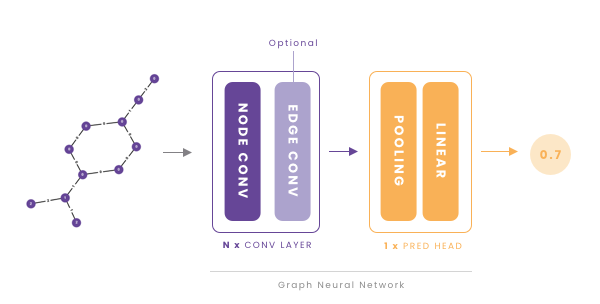
\includegraphics[width=0.45\textwidth]{figures/pipeline.png}
    \caption{High level overview of the model architecture.}
    \label{fig:model}
\end{figure}

At its core, GNN converts a graph into a vector representation for binary classification. 
This work explores two approaches: one using node features and the other incorporating both node and edge features. 
Figure \ref{fig:model} depicts the model architecture. After convolutional layers, node features are reduced using \texttt{MaxPool} or \texttt{MeanPool} into a one-dimensional graph representation. 
A linear layer then produces the final prediction.

\subsection{Node features}
Node feature aggregation employs three types of convolutional layers: 
Normal Graph Convolution (\texttt{NORM}), GraphSAGE (\texttt{SAGE}), 
and Graph Attention (\texttt{GATT}). In \texttt{NORM}, each node's representation 
is computed by aggregating neighbor features, followed by linear transformation and addition.
\texttt{SAGE} extends \texttt{NORM} by offering flexibility in the choice of aggregation function. 
This study utilizes the \texttt{SUM} strategy for efficient and effective aggregation.
Finally, the \texttt{GATT} aggregates the neighbors using attention weights (learnt during training), 
which indicate the importance of each neighbor for the representation of the node. For each neighbor,
the attention weight is computed as a dot product between the trainable vector and concatenation of
the node and neighbor features. Importantly, the \texttt{GATTGl} normalizes the attention weights
using the softmax function over all graph's attention weights, while \texttt{GATTLc} uses the softmax
over the attention weights of the neighbors of the given node. Consequently, the global approach
will only emphasize the most important interactions in the graph, while the local approach focuses
on the most important interactions within the neighborhood.

\subsection{Edge features integration}
As shown in Figure \ref{fig:model}, each node convolution layer is followed by 
an edge convolution, forming a single convolutional block. 
This approach provides flexibility in selecting the edge convolutional layer 
and determining the number of combined convolutional blocks. 
Two types of edge convolutions, namely Edge Sum (\texttt{ESUM}) and Edge Attention (\texttt{EATT}), are compared.

The concept behind \texttt{ESUM} is to update each node's representation by summing the edge features 
associated with the node. Consequently, the node's representation depends not only on its neighbors' types but also on the 
type of connections with its neighbors. The \texttt{EATT} computes the attention weights
as a dot product between each node and edge features. These weights are normalised with respect to 
each node, i.e., the importance of all edges globally for the given node is computed. Finally, \texttt{EATTGl} uses
all edges in the graph, while \texttt{EATTLc} uses only the edges associated with the given node to compute 
the final representation of the given node.


\begin{figure*}
    \centering
    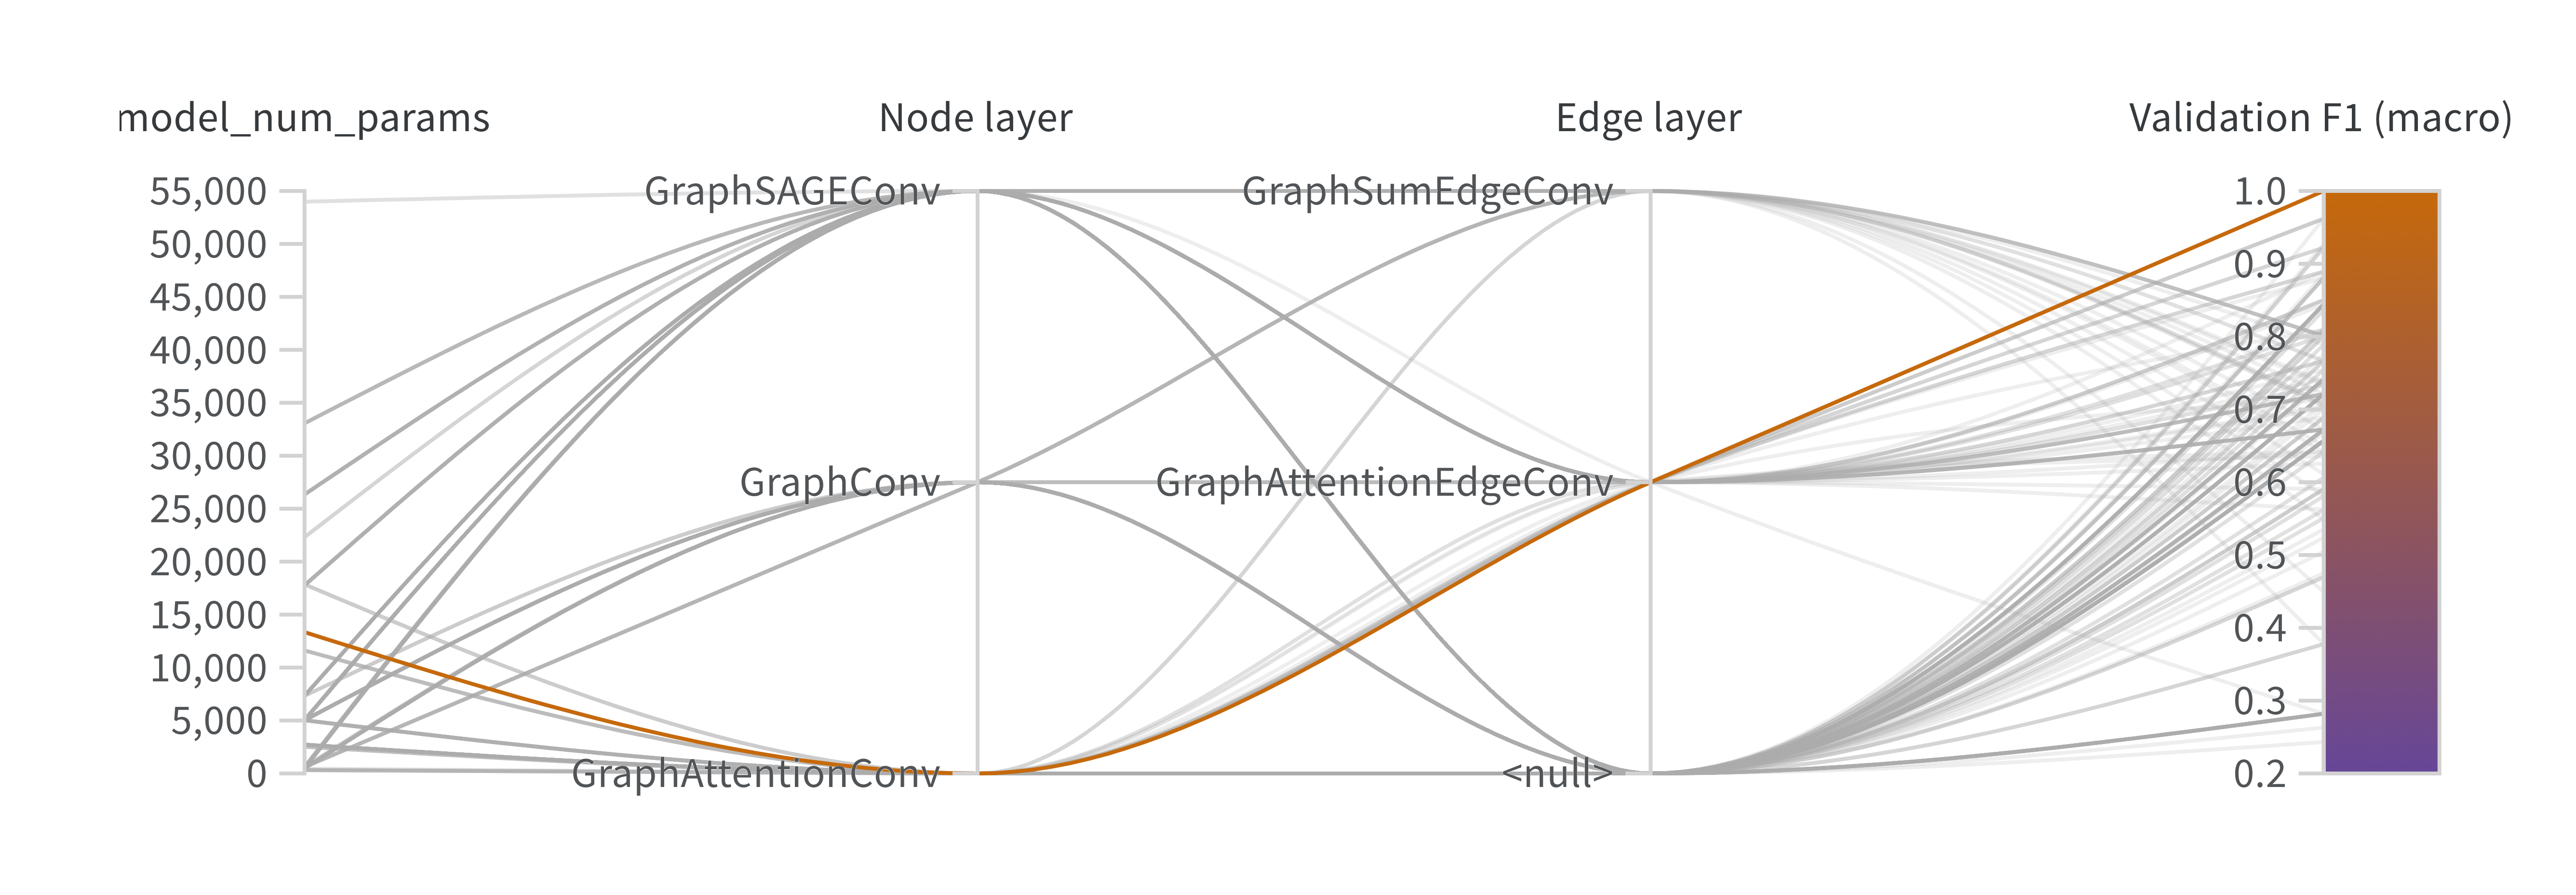
\includegraphics[width=1\textwidth]{figures/hyperparams.png}
    \caption{Relationship between model complexity, type of node and edge convolution and the model's performance. The highlighted line indicates the best performing model.}
    \label{fig:hyperparams}
\end{figure*}

\section{Experiments}
\begin{table}[!ht]
    \centering
    \begin{tabular}{llccc}
    \toprule
    \textbf{Layer} & \textbf{Depth} & \textbf{Loss} & \textbf{F1-Macro} \\
    \midrule
    \texttt{Norm} & M & 0.41 & 0.74 \\
    w/\texttt{EATTGl} & L & 0.32 & 0.85 \\
    \midrule
    \texttt{SAGE} & L & 0.26 & 0.88 \\
    w/\texttt{EATTGl} & L & 0.17 & 0.89 \\
    \midrule
    \texttt{GATTGl} & L & 0.33 & 0.96 \\
    \textbf{w/\texttt{EATTGl}} & \textbf{L} & \textbf{0.19} & \textbf{1.00} \\
    \bottomrule
    \end{tabular}
    \caption{Experiment results evaluated on validation dataset. Depth of the model is indicated by Medium (M, 2 layers) and Large (L, at least 3 layers).}
    \label{tab:results}
\end{table}

Table \ref{tab:results} summarizes experiment results, organized by node convolutional layer type. 
The second row showcases model performance with the better edge feature integration method. 
Notably, the model's performance improves with more sophisticated node convolutional layers, \texttt{GATTGl}
outperforming the other two types. Additionally, most models contain at least three convolutional layers, 
indicating the need for model complexity to learn the task effectively.

As the report's title suggests, enhancing node convolutional layers with aggregated edge features through \texttt{EATTGl} 
consistently boosts performance across all models. The most substantial improvement is observed in the \texttt{Norm} model, 
with a notable 11\% enhancement. While the other two models performed well even without edge features, 
the improvement, while marginal, remains significant.

The top-performing model, \texttt{GATTGl} with \texttt{EATTGl} edge convolution, 
achieved a test set F1-Macro score of 0.77, with an equal number of mispredictions for both classes. 
The notable variation between validation and test scores can likely be attributed in part to the dataset's small 
size and over-tuning of hyperparameters.

\section{Discussion}

\begin{figure}[!ht]
    \centering
    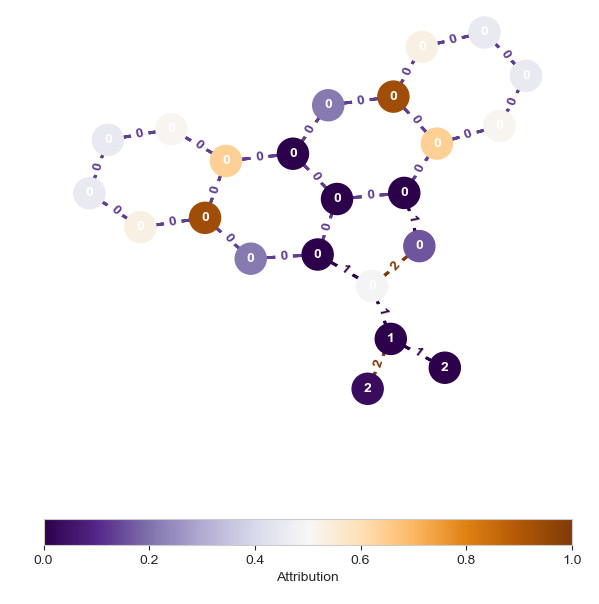
\includegraphics[width=0.35\textwidth]{figures/interpret.png}
    \caption{Visualization of the relative nodes' and edges' importance for the prediction of the graph's label.}
    \label{fig:attribution}
\end{figure}

The results clearly indicate that the attention mechanism is the superior choice for aggregating both node and edge features. 
This aligns with its successful application in various domains \cite{transformers}. 
Notably, for the specific task of mutagenicity prediction, the global approach, which considers all nodes and edges, outperforms the local approach. 
Figure \ref{fig:attribution} provides insight into this phenomenon, illustrating the relative importance of nodes and edges in graph label prediction. 
Integrated Gradients \cite{attribution} is used to compute importance, revealing that the final prediction relies on a selected subset of nodes and edges (orange/brown) 
that don't necessarily need to be directly connected.

Finally, Figure \ref{fig:hyperparams} shows the path to achieving the best-performing models. 
Despite their lower parameter count, attention-based models outperform more complex ones. 
Last but not the least, the weaker performance of models using \texttt{ESUM} for edge aggregation (local approach) 
further underscores the effectiveness of the attention mechanism.

\section{Conclusion}
In conclusion, this report explored the use of Graph Neural Networks for mutagenicity prediction. 
The findings emphasize the significance of both node and edge features in this task. 
Notably, the global attention mechanism emerged as the most effective method for aggregating both types of features. 
Future work may involve evaluating the proposed model on additional datasets and tasks.

\newpage
\bibliographystyle{abbrv}
\bibliography{references}

\end{document}